%! TEX root = ./main.tex

\section{The Model of Carbon Sequestration}
%模型图
The carbon sequestration model can be summarized in in Figure 2.

\begin{figure}[htp]
    \centering
    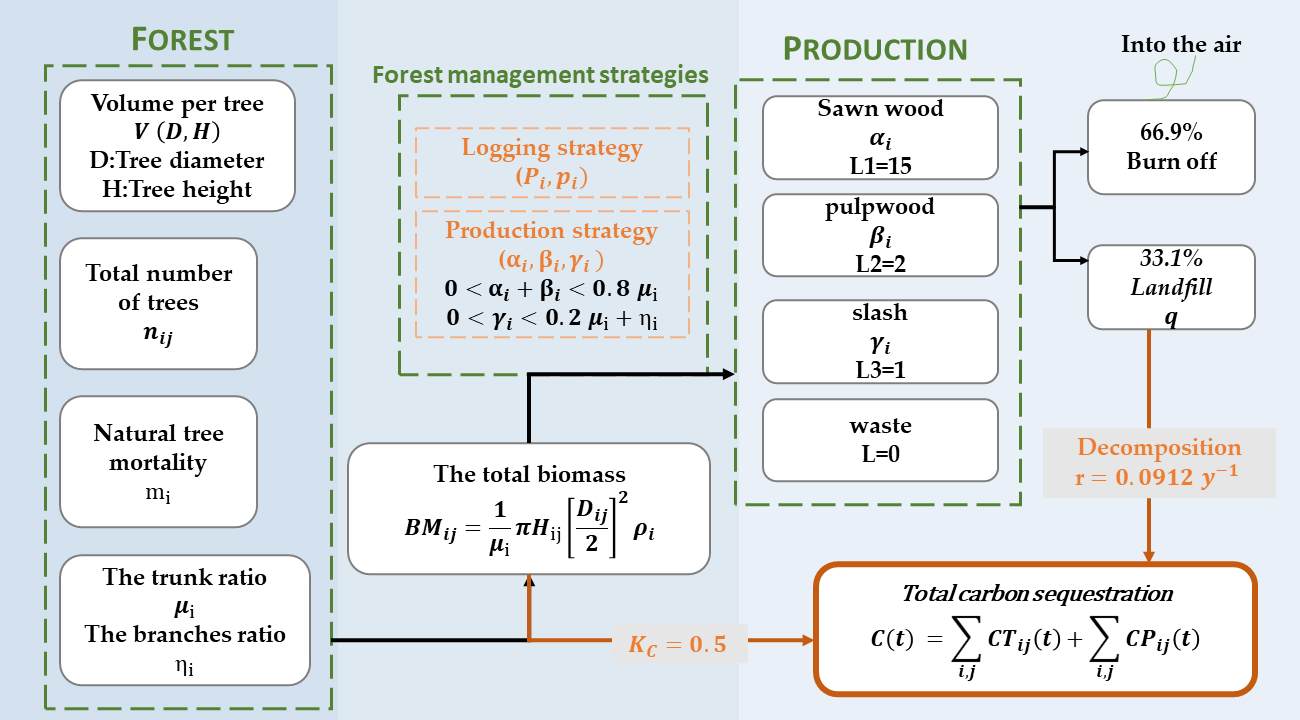
\includegraphics[width=15cm]{figs/Carbon_model.png}
    \caption{Carbon sequestration model.}
    \label{fig:my_label}
\end{figure}

\subsection{Input}

\subsubsection{Biomass function}
Based on the underlying assumptions, we calculate the amount of carbon sequestration by converting the volume of trees into biomass. To calculate the biomass $BM_{ij}$, we first calculated the biomass of the trunk according to the diameter (at breast-height), height and density of the tree, and then calculated the total biomass according to the biomass proportion of the trunk in an individual plant.
\begin{eqnarray}
B M_{i j} & = & \frac{1}{\mu_{i}} \pi H_{i j}\left[\frac{D_{i j}}{2}\right]^{2} \rho_{i}
\end{eqnarray}

It is required that the annual variation data of DBH and height be be collected. The data are used to fit the variation function of tree DBH and tree height, $D_{ij}$ and $H_{ij}$, where $i$ stands for species and $j$ stands for the age. Several S-shaped functions are used for fitting, from which the ones with the best fitting are chosen to represent the variation:
\begin{equation}
\begin{aligned}
    Y&=Kt^{b},\\
    Y&=\frac{t}{a+b t},\\
    Y&=\frac{K}{1+a e^{-bt}},\\
    Y&=K a^{b t},\\
\end{aligned}
\end{equation}
where $K,a,b$ are undetermined constants. With diameter and height functions obtained, the biomass is calculated via formula (1).

\subsubsection{Tree age distribution and tree mortality}
Assuming that the mortality $m_i$ of each species is constant and the total number of trees remains $N_i$, the number of trees of different ages in the current forest can be calculated as follows.
Mark the planting time of the artificial forestation as $T_i$ years ago ($t=-T_i$. Each year, a proportion of $m_i$ was eliminated due to natural death. Dead trees were replaced by new-born trees, controlling the total number to $N_i$. The numbers of trees at $t=0$ are listed below.

\begin{equation}
\begin{array}{c}
n_{i, T_{i}} = N_{i}\left(1-m_{i}\right)^{T_{i}-1} \\
n_{i j} = N_{i} m_{i}\left(i-m_{i}\right)^{j-1}, j = 2,3, \ldots, T_{i}-1 \\
n_{i 1} = N_{i} m_{i}
\end{array}
\end{equation}

Given the average diameter $\overline{D_{i}}$  of each tree species, the natural mortality $m_i$ of trees under the environmental conditions can be obtained by bisection method. And by applying $m_i$, the age distribution of trees at $t=0$ can be obtained using formula (3).

\begin{equation}
\overline{D_{i}}=\frac{\sum_{j=1}^{T_{i}} D_{i j} n_{i j}}{\sum_{j=1}^{T_{i}} n_{i j}}
\end{equation}

\subsubsection{Coefficient of biomass conversion to carbon sequestration}
Forest carbon sequestration is mainly calculated by measuring the biomass of forest vegetation and multiplying it by the biomass - carbon conversion coefficient $K_c$. The 2006 IPCC Guidelines for National GHG Inventories recommended the carbon ratio of aboveground forest biomass. 

To simplify the model, we take $K_c$ as 0.5, which is the average value of empirical data given by IPCC.


\subsubsection{Service life of the product}

Based on the nature of the wood used, we classify forest products into sawn-wood, pulp-wood and slash.The specific definition is as follows.

% \usepackage{colortbl}
\begin{table}[htp]
\caption{Classification of forest products.}
\begin{tabular}{llll} 
\hline
\textbf{Product} & \textbf{Instance}               & \textbf{Service life /year} & \textbf{Disposal mode}                                                                                          \\ 
\hline
sawn-wood        & Furniture,
  building materials & 15                          & Landfill or incineration.                                                   \\
pulp-wood        & Plywood,
  cardboard, paper     & 10~                         & Landfill or incineration. \\
Slash            & Fuel                            & 1                           & Burned.                                                                                                         \\
\hline
\end{tabular}
\end{table}

The average product life $L_1$ of Sawn-wood is assumed to be 15 years, the life $L_2$ of pulp-wood is assumed to be 10 years, and the life $L_3$ of slash is assumed to be 1 year. The discarded part has no service life and is not included in the calculation system.

\subsubsection{Landfill and decomposition parameters}
We divided the final destination of forest products into landfill and incineration. Any treatment other than landfill is treated as incineration, which releases CO$_2$ directly into the air and does not count in the carbon sequestration system.

According to the \emph{2020 Annual Report on The Prevention and Control of Environmental Pollution by Large and medium-sized Cities} released by the Ministry of Ecology and Environment of China, the current landfill rate $q$ in China is 33.1\%, and the decomposition rate $r$ is 0.0912 per year\cite{Decomposition_rate}. The carbon sequestration effect of these forest products is included in the calculation system.

\subsection{Calculation carbon sequestration}
\subsubsection{Variation of age distribution}
The tree age distribution of each year from $t=0$ is obtained by iteration. The relationship between the age distribution of trees in the two adjacent years is

\begin{equation}
\begin{aligned}
    n_{i1}(t+1)&=N_i m_i + \sum_{j>P_i}n_{i j}\times(1-m_i)\timesp_i \\
    n_{i j}(t+1)&=n_{i j}(t)\times(1-m_i),1<j<P_i\\
    n_{i j}(t+1)&=n_{i j}(t)\times(1-m_i)\times(1-p_i),j\ge P_i\\
\end{aligned}
\end{equation}

Formula (5) means that trees that were dead or cut down would be replaced by new-born trees in the next year.

\subsubsection{Carbon sequestration in trees}

The carbon sequestration in trees can be converted from biomass of living trees.

\begin{equation}
    CT_i(t) = K_C\times \sum_{j}BM_ij\times n_{ij}(t)
\end{equation}

\subsubsection{Carbon sequestration in products}
For each year, the biomass of cut-down trees in species $i$ is
\begin{equation}
    H_i(t)=\sum_{j>P_i}n_{ij}(t)\times p_i\timesBM_{ij}
\end{equation}
The biomass percentage of trees that are made into sawn-wood, pulpwood and slash are respectively $\alpha_i,\beta_i,\gamma_i$, their service lives being $L_1,L_2,L_3$. A proportion of $q$ for sawn-wood and pulpwood ends up in landfill. The decomposing rate in landfill is $r$. Therefore, the carbon sequestration in products and its wastes comply with the following relationship:

\begin{equation}
\begin{aligned}
    \frac{CP_i(t)}{K_C}=&\sum_{\Delta t=0}^{L_1}H_i(t-\Delta t)\times \alpha_i+\sum_{\Delta t=0}^{L_2}H_i(t-\Delta t)\times \beta_i+\sum_{\Delta t=0}^{L_3}H_i(t-\Delta t)\times \gamma_i\\
    &+\sum_{\Delta t=L_1}^{\infty}H_i(t-\Delta t)\times \alpha_i\times e^{-r(\Delta t-L_1)}+\sum_{\Delta t=L_2}^{\infty}H_i(t-\Delta t)\times \beta_i\times e^{-r(\Delta t-L_2)}
\end{aligned}
\end{equation}

\subsection{Management strategies}
\subsubsection{Logging strategy}
Logging strategy is an important part of forest management strategy, which directly affects the balance between forest and forest products. We introduce a logging strategy (p$_i$,P$_i$). This means that for every tree species $i$, a proportion equal to $p_{i}$ of trees should be cut down for trees older than the age of rotation period $P_i$.

By default, $p_i$ varies continuously between 0 and 1. For simplicity, we set $p_i$  to the same for each tree species.

Based on actual forest farm data, we tested the changes in carbon sequestration resulting from different logging strategies.

\subsubsection{Production strategy}
Forest products are divided into three categories according to their wood properties -- sawn-wood, pulp-wood and slash. They are represented by $\alpha_i$, $\beta_i$ and $\gamma_i$ respectively. Product strategies can be described by number pairs ($\alpha_i$, $\beta_i$, $\gamma_i$). The waste in the production process is treated as a product with a life cycle of 0, which means rapid and complete decomposition within a year.

The biomass of the trunk of the whole tree is $\mu_i$, and the biomass of the branches is $\eta_i$. Assuming 80\% of the trunk can be made into sawn-wood, the rest of the trunk and branches can be made into pulpwood or slash. Everything else was discarded. We derive the following inequality to generalize the state of production.
\begin{equation}
\begin{array}{c}
0<\alpha_{i}+\beta_{i}<0.8 \mu_{i} \\
0<\gamma_{i}< \mu_{i}+\eta_{i} \\
\end{array}
\end{equation}

To simplify the model, the production strategy takes two extremes:

1.$\left(\alpha_{i}, \beta_{i}, \gamma_{i}\right)=\left(0.8 \mu_{i}, 0.2 \mu_{i}+\eta_{i}, 0\right)$

2.$\left(\alpha_{i}, \beta_{i}, \gamma_{i}\right)=\left(0, \mu_{i}, \eta_{i}\right)$

The former is the most conducive to carbon sequestration distribution, that is, to achieve the longest life of the product. The latter is the most unfavorable to carbon sequestration. Any other situation should be in between the two.

\subsection{Output}
In the above carbon sequestration model, carbon sequestration is divided into forest carbon sequestration and forest product carbon sequestration. The parameters can be used to calculate the carbon sequestration of each forest by fitting the actual forest farm data.
\begin{equation}
\begin{array}{c}

C(t)=\sum_{i,j}CT_{i}(t)+\sum_{i}CP_{i}(t)

\end{array}
\end{equation}